\documentclass{beamer}
\usepackage[utf8]{inputenc}
\usepackage{tikz}
\usepackage[framemethod=tikz]{mdframed}

\usetikzlibrary{positioning,shapes,fit,arrows}
\graphicspath{ {./images/} }

% \usepackage{color}
% \usepackage{listings}
% % Default fixed font does not support bold face
% \DeclareFixedFont{\ttb}{T1}{txtt}{bx}{n}{9} % for bold
% \DeclareFixedFont{\ttm}{T1}{txtt}{m}{n}{9}  % for normal

% % Custom colors
% \usepackage{color}
% \definecolor{deepblue}{rgb}{0,0,0.5}
% \definecolor{deepred}{rgb}p
% \definecolor{deepgreen}{rgb}{0,0.5,0}

% % Python style for highlighting
% \newcommand\pythonstyle{\lstset{
% language=Python,
% basicstyle=\ttm,
% otherkeywords={self},             % Add keywords here
% keywordstyle=\ttb\color{deepblue},
% emph={MyClass,__init__},          % Custom highlighting
% emphstyle=\ttb\color{deepred},    % Custom highlighting style
% stringstyle=\color{deepgreen},
% frame=tb,                         % Any extra options here
% showstringspaces=false            % 
% }}


% % Python environment
% \lstnewenvironment{python}[1][]
% {
% \pythonstyle
% \lstset{#1}
% }
% {}

% % Python for external files
% \newcommand\pythonexternal[2][]{{
% \pythonstyle
% \lstinputlisting[#1]{#2}}}

% % Python for inline
% \newcommand\pythoninline[1]{{\pythonstyle\lstinline!#1!}}


\usepackage{xcolor}
\definecolor{maroon}{cmyk}{0, 0.87, 0.68, 0.32}
\definecolor{halfgray}{gray}{0.55}
\definecolor{ipython_frame}{RGB}{207, 207, 207}
\definecolor{ipython_bg}{RGB}{247, 247, 247}
\definecolor{ipython_red}{RGB}{186, 33, 33}
\definecolor{ipython_green}{RGB}{0, 128, 0}
\definecolor{ipython_cyan}{RGB}{64, 128, 128}
\definecolor{ipython_purple}{RGB}{170, 34, 255}

\usepackage{listings}
\lstset{
    breaklines=true,
    %
    extendedchars=true,
    literate=
    {á}{{\'a}}1 {é}{{\'e}}1 {í}{{\'i}}1 {ó}{{\'o}}1 {ú}{{\'u}}1
    {Á}{{\'A}}1 {É}{{\'E}}1 {Í}{{\'I}}1 {Ó}{{\'O}}1 {Ú}{{\'U}}1
    {à}{{\`a}}1 {è}{{\`e}}1 {ì}{{\`i}}1 {ò}{{\`o}}1 {ù}{{\`u}}1
    {À}{{\`A}}1 {È}{{\'E}}1 {Ì}{{\`I}}1 {Ò}{{\`O}}1 {Ù}{{\`U}}1
    {ä}{{\"a}}1 {ë}{{\"e}}1 {ï}{{\"i}}1 {ö}{{\"o}}1 {ü}{{\"u}}1
    {Ä}{{\"A}}1 {Ë}{{\"E}}1 {Ï}{{\"I}}1 {Ö}{{\"O}}1 {Ü}{{\"U}}1
    {â}{{\^a}}1 {ê}{{\^e}}1 {î}{{\^i}}1 {ô}{{\^o}}1 {û}{{\^u}}1
    {Â}{{\^A}}1 {Ê}{{\^E}}1 {Î}{{\^I}}1 {Ô}{{\^O}}1 {Û}{{\^U}}1
    {œ}{{\oe}}1 {Œ}{{\OE}}1 {æ}{{\ae}}1 {Æ}{{\AE}}1 {ß}{{\ss}}1
    {ç}{{\c c}}1 {Ç}{{\c C}}1 {ø}{{\o}}1 {å}{{\r a}}1 {Å}{{\r A}}1
    {€}{{\EUR}}1 {£}{{\pounds}}1
}

%%
%% Python definition (c) 1998 Michael Weber
%% Additional definitions (2013) Alexis Dimitriadis
%% modified by me (should not have empty lines)
%%
\lstdefinelanguage{iPython}{
    morekeywords={access,and,break,class,continue,def,del,elif,else,except,exec,finally,for,from,global,if,import,in,is,lambda,not,or,pass,print,raise,return,try,while},%
    %
    % Built-ins
    morekeywords=[2]{abs,all,any,basestring,bin,bool,bytearray,callable,chr,classmethod,cmp,compile,complex,delattr,dict,dir,divmod,enumerate,eval,execfile,file,filter,float,format,frozenset,getattr,globals,hasattr,hash,help,hex,id,input,int,isinstance,issubclass,iter,len,list,locals,long,map,max,memoryview,min,next,object,oct,open,ord,pow,property,range,raw_input,reduce,reload,repr,reversed,round,set,setattr,slice,sorted,staticmethod,str,sum,super,tuple,type,unichr,unicode,vars,xrange,zip,apply,buffer,coerce,intern},%
    %
    sensitive=true,%
    morecomment=[l]\#,%
    morestring=[b]',%
    morestring=[b]",%
    %
    morestring=[s]{'''}{'''},% used for documentation text (mulitiline strings)
    morestring=[s]{"""}{"""},% added by Philipp Matthias Hahn
    %
    morestring=[s]{r'}{'},% `raw' strings
    morestring=[s]{r"}{"},%
    morestring=[s]{r'''}{'''},%
    morestring=[s]{r"""}{"""},%
    morestring=[s]{u'}{'},% unicode strings
    morestring=[s]{u"}{"},%
    morestring=[s]{u'''}{'''},%
    morestring=[s]{u"""}{"""},%
    %
    % {replace}{replacement}{lenght of replace}
    % *{-}{-}{1} will not replace in comments and so on
    literate=
    {á}{{\'a}}1 {é}{{\'e}}1 {í}{{\'i}}1 {ó}{{\'o}}1 {ú}{{\'u}}1
    {Á}{{\'A}}1 {É}{{\'E}}1 {Í}{{\'I}}1 {Ó}{{\'O}}1 {Ú}{{\'U}}1
    {à}{{\`a}}1 {è}{{\`e}}1 {ì}{{\`i}}1 {ò}{{\`o}}1 {ù}{{\`u}}1
    {À}{{\`A}}1 {È}{{\'E}}1 {Ì}{{\`I}}1 {Ò}{{\`O}}1 {Ù}{{\`U}}1
    {ä}{{\"a}}1 {ë}{{\"e}}1 {ï}{{\"i}}1 {ö}{{\"o}}1 {ü}{{\"u}}1
    {Ä}{{\"A}}1 {Ë}{{\"E}}1 {Ï}{{\"I}}1 {Ö}{{\"O}}1 {Ü}{{\"U}}1
    {â}{{\^a}}1 {ê}{{\^e}}1 {î}{{\^i}}1 {ô}{{\^o}}1 {û}{{\^u}}1
    {Â}{{\^A}}1 {Ê}{{\^E}}1 {Î}{{\^I}}1 {Ô}{{\^O}}1 {Û}{{\^U}}1
    {œ}{{\oe}}1 {Œ}{{\OE}}1 {æ}{{\ae}}1 {Æ}{{\AE}}1 {ß}{{\ss}}1
    {ç}{{\c c}}1 {Ç}{{\c C}}1 {ø}{{\o}}1 {å}{{\r a}}1 {Å}{{\r A}}1
    {€}{{\EUR}}1 {£}{{\pounds}}1
    %
    {^}{{{\color{ipython_purple}\^{}}}}1
    {=}{{{\color{ipython_purple}=}}}1
    %
    {+}{{{\color{ipython_purple}+}}}1
    {*}{{{\color{ipython_purple}$^\ast$}}}1
    {/}{{{\color{ipython_purple}/}}}1
    %
    {+=}{{{+=}}}1
    {-=}{{{-=}}}1
    {*=}{{{$^\ast$=}}}1
    {/=}{{{/=}}}1,
    literate=
    *{-}{{{\color{ipython_purple}-}}}1
     {?}{{{\color{ipython_purple}?}}}1,
    %
    identifierstyle=\color{black}\ttfamily,
    commentstyle=\color{ipython_cyan}\ttfamily,
    stringstyle=\color{ipython_red}\ttfamily,
    keepspaces=true,
    showspaces=false,
    showstringspaces=false,
    %
    rulecolor=\color{ipython_frame},
    frame=single,
    frameround={t}{t}{t}{t},
    framexleftmargin=6mm,
    numbers=left,
    numberstyle=\tiny\color{halfgray},
    %
    %
    backgroundcolor=\color{ipython_bg},
    %   extendedchars=true,
    basicstyle=\scriptsize,
    keywordstyle=\color{ipython_green}\ttfamily,
}

% \definecolor{light-gray}{gray}{0.95}
\surroundwithmdframed[
  hidealllines=true,
  innerleftmargin=15pt,
  innertopmargin=0pt,
  innerbottommargin=0pt]{lstlisting}

\usetheme{Berlin}
\usefonttheme[onlymath]{serif}

% \usecolortheme{crane}
\setbeamertemplate{navigation symbols}{}%remove navigation symbols

\title[Stacks and Queues]{\textbf{Stacks and Queues}}
\subtitle{A Brief Introduction}
% \author{Shon Verch}
\institute{Stephen Lewis Secondary School}
\author{Computer Science Club}
\date{December 7, 2018}

\newcommand{\sectionFrame}[3]
{
    \section{#3}
    \begin{frame}
    \begin{block}{}
    \begin{center}
        \Huge{#1}\\[0.5ex]
        \large{#2}
    \end{center}
    \end{block}
    \end{frame}
}

\usepackage{caption}

\begin{document}
\begin{frame} 
\titlepage 
\end{frame}

\section{Introduction}
\subsection{Abstraction}
\begin{frame}{Premise}
The following lecture deals with a branch of computer science called \textit{data structures}. In particular, we will explore two fundamental data structures:
\begin{itemize}
    \item Stacks
    \item Queues
\end{itemize}

\end{frame}

\begin{frame}{Data Type}
A \textit{data type} is a set of values and a set of operations on those values (data and logic).

\begin{block}{Example}
In Python, an \lstinline[language=iPython]{int} is a primitive data type; the values include all the integers;\footnote[frame]{Python integers are unbounded; they have no min or max size.} the operations include $+$, $-$, $*$, $/$, $\%$, $<$, and $>$.
\end{block}
\end{frame}

\begin{frame}{Data Abstraction}
Earlier, we discussed the concept of \textit{object-oriented programming} and we used it to define ``classes'' that contain a set of related data and logic.\\~\\
Abstraction builds on this principle to hide logic from the client. An abstract data type is a data type whose implementation and representation are hidden from the client.\footnote[frame]{The ``client'' refers to the code that is using the data type (i.e. a fellow programmer).}
\end{frame}

\begin{frame}{What's the point?}

Abstraction allows us to create \textbf{generalised} code.\\~\\
When we \textit{use} an ADT, we focus on the operations specified by the data type and pay no attention to the underlying implementation.\\~\\

When we \textit{implement} an ADT, we focus on the data, and then implement operations that use the data.
\end{frame}

\section{Stacks}
\subsection{Introduction}
\begin{frame}{What is a stack?}

The stack ADT stores objects in a last-in-first-out scheme (LIFO). It mirrors a physical stack (e.g. a stack of plates).\\~\\
Adding and removing elements is restricted; at any time, only the top element can be removed from the stack---we cannot remove elements from the middle of the stack.
\end{frame}

\subsection{ADT Design}
\begin{frame}{Primary Operations}
A stack has two primary operations:
\begin{itemize}
    \item \textbf{push}: inserts an element onto the top of the stack
    \item \textbf{pop}: removes and returns the top element from the stack
\end{itemize}
\end{frame}

\begin{frame}[fragile]{Pushing an element}
\begin{columns}
    \column{0.7\linewidth}
    The stack is stored as a list. Implementing the push operation is as simple as adding the item to the end of the list.
    \begin{center}
    \begin{lstlisting}[language=iPython]
def push(self, item):
    return self.buffer.append(item)\end{lstlisting}
    \end{center}
    \column{0.3\linewidth}
    \centering
    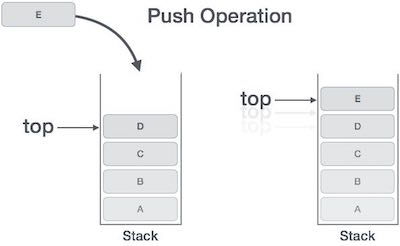
\includegraphics[width=3.5cm]{lessons/images/stack_push_operation.jpg}
\end{columns}
\end{frame}

\begin{frame}[fragile]{Popping an element}
\begin{columns}
    \column{0.7\linewidth}
    Implementing the pop operation is \textit{very} simple because Python lists come with a built-in \lstinline[language=iPython]{pop} method.
    \begin{center}
    \begin{lstlisting}[language=iPython]
def pop(self):
    return self.buffer.pop()\end{lstlisting}
    \end{center}
    \column{0.3\linewidth}
    \centering
    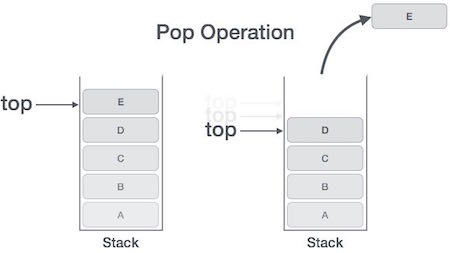
\includegraphics[width=3.5cm]{lessons/images/stack_pop_operation.jpg}
\end{columns}
\end{frame}

\section{Queues}
\subsection{Introduction}
\begin{frame}{What is a queue?}
    
The queue ADT stores objects in a first-in-first-out scheme (FIFO). It is similar to a queue of people at an amusement park (e.g. a lineup).
\\~\\
Like a stack, adding and removing elements is restricted; at any time, only the first element can be removed from the queue.
\end{frame}

\subsection{ADT Design}
\begin{frame}{Primary Operations}
A queue has two primary operations:
\begin{itemize}
    \item \textbf{enqueue}: inserts an element to the back of the queue
    \item \textbf{dequeue}: removes and returns the first element in the queue
\end{itemize}
\end{frame}

\begin{frame}[fragile]{Enqueuing an element}
\begin{columns}
    \column{1\linewidth}
    The queue is stored as a list. Implementing the enqueue operation is as simple as adding the item to the \textit{front} of the list.
    \begin{center}
    \begin{lstlisting}[language=iPython]
def enqueue(self, item):
    # insert the item at the 0-th index.
    return self.buffer.insert(0, item)\end{lstlisting}
    \end{center}
\end{columns}
\end{frame}

\begin{frame}[fragile]{Dequeuing an element}
\begin{columns}
    \column{1\linewidth}
    The \lstinline[language=iPython]{pop} method removes the last item in the list. Since we are adding new elements to the front of the list, the last element in the list is the oldest.
    \begin{center}
    \begin{lstlisting}[language=iPython]
def dequeue(self):
    return self.buffer.pop()\end{lstlisting}
    \end{center}
\end{columns}
\end{frame}

\subsection{Python Queues}
\begin{frame}[fragile]{The Queue Module}
\begin{columns}
    \column{1\linewidth}
    Python includes a built-in Queue library which is recommended for most purposes.\\~\\
    The enqueue operation is \lstinline[language=iPython]{put(item)} and the dequeue operation is \lstinline[language=iPython]{get()}.
    \begin{center}
    \begin{lstlisting}[language=iPython]
from queue import Queue

# create the queue
q = Queue()
q.put(5) # enqueue an item

i = q.get() # i = 5; q is empty \end{lstlisting}
    \end{center}
\end{columns}

\end{frame}

% \begin{frame}[fragile]{Interface}
% \begin{columns}
%     \begin{column}{0.3\textwidth}
%         %Content
%     \end{column}
%     \begin{column}{0.7\textwidth}
%     \begin{lstlisting}
%     class Stack:
%         def __init__(self):
%     \end{lstlisting}
%     \end{column}
% \end{columns}
% \end{frame}

\end{document}